% Text for chapter 1
\chapter{Introduction}\label{ch:introduction}

% Figure manager for Chapter 1
% spell-checker: disable
\begin{pycode}[chapter1]
name = 'chapter1'
ch1 = texfigure.Manager(
    pytex,
    os.path.join('.', name),
    number=1,
    **{k: os.path.join('.', name, v) for k,v in manager_opts.items()}
)
from matplotlib.path import Path
import matplotlib.patches

from formatting import remove_ticks_and_spines
\end{pycode}
% spell-checker: enable

% lead with description of the 2017 eclipse
% transition to discussion of ancient eclipse observations
% sun affects us everyday: life, space weather, analogue for other stars

\section{The Structure of the Solar Atmosphere}

% diagram of structure of the corona

%\subsection{Interior}
%
%\subsubsection{Core}
%\subsubsection{Radiative Zone}
%\subsubsection{Convection Zone}
%
%\subsection{Photosphere}

% three panel figure with 4500, 304, 131/193 showing transition from photosphere to chromosphere to corona
%
%\subsection{Chromosphere}
%
%\subsection{Transition Region}
%
%\subsection{Corona}

% characteristics of the corona
% discuss EUV and X-ray observations of the corona (ref figure)

% spell-checker: disable %
\begin{pycode}[chapter1]
# Import all maps
maps = []
instrs = [ 'sxt', 'eit', 'xrt', 'aia' ]
for i in instrs:
    maps.append(Map(os.path.join(ch1.data_dir, f'{i}_example.fits' )))
# Fix XRT metadata
maps[2] = Map(maps[2].data,{**maps[2].meta,
                        'wavelnth': f'{maps[2].meta["ec_fw1_"]}/{maps[2].meta["ec_fw2_"]}'})
# Set colormap normalization
for m in maps:
    m.plot_settings['norm'] = ImageNormalize(vmin=max(0,m.data.min()),
                                             vmax=m.data.max(),
                                             stretch=LogStretch())
maps[-1].plot_settings['norm'] = ImageNormalize(vmin=max(0, maps[-1].data.min()),
                                                vmax=maps[-1].data.max()*0.25,
                                                stretch=AsinhStretch(0.1))

# Make figure
fig = plt.figure(figsize=texfigure.figsize(
    pytex,
    scale=1,
    height_ratio=1,
))
for i,m in enumerate(maps):
    ax = fig.add_subplot(2, 2, i+1, projection=m)
    m.plot(axes=ax,annotate=False,)
    ax.grid(alpha=0)
    lon,lat = ax.coords[0],ax.coords[1]
    lon.set_ticks_visible(False)
    lon.set_ticklabel_visible(False)
    lat.set_ticks_visible(False)
    lat.set_ticklabel_visible(False)
    lon.frame.set_linewidth(0)
    lat.frame.set_linewidth(0)
    try:
        wvl = m.meta['wavelnth'] * u.Angstrom
        wvl = f"{m.meta['wavelnth']} {u.Angstrom.to_string(format='latex')}"
    except ValueError:
        wvl = m.meta['wavelnth']
    ax.text(0, m.dimensions.y.value-10,
            f'{m.observatory}/{m.instrument.split(" ")[0]} {wvl}',
            color='w',
            fontsize=plt.rcParams['legend.fontsize']*0.75,
            horizontalalignment='left',
            verticalalignment='top',)
    ax.text(m.dimensions.x.value,0,
            astropy.time.Time(m.date).strftime('%Y/%d/%m'),
            color='w',
            fontsize=plt.rcParams['legend.fontsize']*0.75,
            horizontalalignment='right',
            verticalalignment='bottom')
plt.subplots_adjust(hspace=0.01,wspace=0.01)

# Save figure
tfig = ch1.save_figure('example-images', fext='.pdf')
tfig.caption = r''
\end{pycode}
\py[chapter1]|tfig|
% spell-checker: enable %

%\subsection{Solar Wind}

% very briefly

\section{The Solar Magnetic Field}

% comment on beta, frozen-in flux condition

\subsection{Flux Emergence}

% dynamo, flux emergence, formation of ARs (define AR)

\subsection{Observations}

% comments on how we observe magnetic fields in the corona (Zeeeman, Hanle)
% LOS vs vector magnetograms
% show a synoptic map (GONG) or full-disk (HMI)

\subsection{Field Extrapolation}\label{sec:field_extrapolation}

In general, determining the vector magnetic field in the corona requires solving the coupled, non-linear equations of \textit{magnetohydrodynamics} (MHD),
\begin{align}
    &\frac{d}{dt}\rho + \rho\nabla\cdot\mathbf{v} = 0, \label{eq:mhd_continuity} \\
    &\rho\frac{d}{dt}\mathbf{v} = \frac{1}{c}\mathbf{j}\times\mathbf{B} - \nabla p, \label{eq:mhd_momentum} \\
    &\mathbf{j} = \frac{c}{4\pi}\nabla\times\mathbf{B}, \label{eq:mhd_ampere} \\
    &\frac{\partial}{\partial t}\mathbf{B} = \nabla\times(\mathbf{v}\times\mathbf{B}) + \frac{\eta c^2}{4\pi}\nabla^2\mathbf{B}, \label{eq:mhd_faraday} \\
    &\nabla\cdot\mathbf{B} = 0, \label{eq:mhd_divb} \\
    &\frac{\rho^\gamma}{\gamma - 1}\frac{d}{dt}\left(\frac{p}{\rho^{\gamma}}\right) = -\nabla\cdot\mathbf{q} - R + H, \label{eq:mhd_energy}
\end{align}
where $\rho$ is the mass density, $\mathbf{v}$ is the bulk flow velocity, $\mathbf{j}$ is the current density, $\mathbf{B}$ is the magnetic field, $p$ is the thermal pressure, $\eta$ is the magnetic diffusivity, $\gamma=5/3$ is the ratio of specific heats, $\mathbf{q}$ is the heat flux, $R$ is the radiative loss term, $H$ is heating due to Ohmic and viscous dissipation, and $d/dt\equiv\partial/\partial t + \mathbf{v}\cdot\nabla$ \citep{priest_magnetohydrodynamics_2014}. Solving the MHD equations for the time-dependent, vector magnetic field in three-dimensions is an extremely challenging problem that requires sophisticated numerical tools and significant computational resources. However, several methods exist for efficiently approximating the coronal magnetic field in \textit{magnetohydrostatic equilibrium} given an observation of the photospheric LOS magnetic field.

\textit{Magnetic field extrapolation} is a commonly-used technique for approximating the three-dimensional vector magnetic field in the corona. Following the treatment in \citet[Chapter 3]{priest_magnetohydrodynamics_2014}, \autoref{eq:mhd_momentum}, the ideal MHD momentum equation, in magnetohydrostatic balance can be written as,
\begin{equation}\label{eq:magnetohydrostatic_balance}
    0 = \frac{1}{c}\mathbf{j}\times\mathbf{B} - \nabla p.
\end{equation}
In a low-$\beta$ plasma where the magnetic pressure dominates over the thermal pressure (see \autoref{ch:loops}), the first term on the right-hand side can often be neglected such that \autoref{eq:magnetohydrostatic_balance} becomes,
\begin{equation}\label{eq:force_free}
    \mathbf{j}\times\mathbf{B} = 0.
\end{equation}
\autoref{eq:force_free} is the so-called \textit{force-free} condition. Combined with \autoref{eq:mhd_ampere}, Amp\'{e}re's law, this implies that,
\begin{equation}\label{eq:ampere_force_free}
    \nabla\times\mathbf{B} = \alpha\mathbf{B},
\end{equation}
where, in general, the scalar $\alpha$ may be some function of position $\mathbf{r}$.

In the case of $\alpha=0$, $\mathbf{j}=0$ (from \autoref{eq:mhd_ampere}) and the magnetic field is said to be current-free or \textit{potential}. \autoref{eq:ampere_force_free} implies that $\mathbf{B}$ is also curl-free such that it can be expressed as,
\begin{equation}\label{eq:b_potential}
    \mathbf{B}=\nabla\phi,
\end{equation}
 where $\phi$ is some scalar potential. Combining this expression with the requirement from Maxwell's equations that the magnetic field must always be divergence-free (\autoref{eq:mhd_divb}) gives Laplace's equation,
\begin{equation}\label{eq:laplace}
    \nabla^2\phi = 0.
\end{equation}
If the normal component of the magnetic field is specified on the lower boundary (e.g. from a photospheric LOS magnetogram), the solution within a closed volume is unique \citep{priest_magnetohydrodynamics_2014}.

Several methods have been developed to solve \autoref{eq:laplace} for the coronal magnetic field. The potential field source surface (PFSS) model of \citet{schatten_model_1969} solves \autoref{eq:laplace} for the global corona given a synoptic photospheric magnetogram as the lower boundary input and under the assumption that the field is purely radial at some ``source surface'', typically $2.5R_{\solar}$. Additionally, the Green's function method of \citet{schmidt_observable_1964} can be used to efficiently determine the potential magnetic field on the scale of a single \AR{} on a Cartesian grid given a LOS magnetogram. \autoref{sec:potential_field} will describe the latter method in detail. While the work presented in this thesis will only make use of photospheric LOS magnetogram data, there exist many techniques for computing field extrapolations from vector magnetograms as well \citep[see review by][]{welsch_deriving_2016}.

The potential field represents the lowest possible energy state of the magnetic field and is likely to be an appropriate approximation provided the magnetic energy dominates over the thermal energy ($\beta<1$) and the field has had sufficient time to relax to the lowest energetic state \citep{priest_magnetohydrodynamics_2014}. Thus, a field with a non-zero current is in a higher energy state than a potential field. From \autoref{eq:mhd_ampere}, if $\mathbf{j}\neq0$ then $\alpha\neq0$. Provided \autoref{eq:force_free} holds, solutions to \autoref{eq:ampere_force_free} represent non-potential force-free fields and in general are much more difficult to compute than potential field solutions. If $\alpha$ is constant, the solution is a linear force-free field, but if $\alpha$ is a function of a position $\mathbf{r}$, the magnetic field is said to be non-linear force-free. See \citet{wiegelmann_solar_2012} for a comprehensive review of force-free magnetic fields in solar physics.

\subsection{Reconnection}\label{sec:reconnection}

After the magnetic field is forced into the solar atmosphere by the bouyant motion of the convective zone, it remains rooted in the photosphere, whether it is \textit{open} (flux tube extends radially outward, possibly connecting with the interplanetary magnetic field) or \textit{closed} (both ends attached to the solar surface). Because the field is \textit{line-tied}, or frozen into the photospheric plasma, the turbulent motion of the photosphere deforms and stresses the overlying field, leading to the storage of magnetic energy. This motion can eventually lead to a topological restructuring of the magnetic field as it relaxes from a stressed to an equilibrium state, a process commonly referred to as \textit{magnetic reconnection}.

% spell-checker: disable %
\begin{pycode}[chapter1]
arrow_style = {
    'lw': 3,
    'head_width': 0.0125,
    'head_length': 0.01,
    'edgecolor': 'k',
    'facecolor': 'k'
}
dot_style = { 'marker': 'o', 'markersize': 7.5, 'ls': ''}

fig = plt.figure(figsize=texfigure.figsize(
    pytex,
    scale=1,
    height_ratio=2/5,
))

# Panel 1
ax = fig.add_subplot(131)
ax.set_aspect(aspect=1.5)
ax.set_xlim(-0.1,1.1)
ax.set_ylim(-0.1,1.1)
remove_ticks_and_spines(ax)
# First curve
patch = matplotlib.patches.PathPatch(
    Path([(0,0),(0.6,0.5),(0,1),], [Path.MOVETO,Path.CURVE3,Path.CURVE3,]),
    facecolor='none', edgecolor=DEEP_PALETTE[3], lw=2)
ax.add_patch(patch)
ax.plot([0,0], [0,1], **dot_style, color=DEEP_PALETTE[3])
# Second curve
patch = matplotlib.patches.PathPatch(
    Path([(1,0),(0.4,0.5),(1,1),], [Path.MOVETO,Path.CURVE3,Path.CURVE3,]),
    facecolor='none',edgecolor=DEEP_PALETTE[0],lw=2)
ax.add_patch(patch)
ax.plot([1,1],[0,1], **dot_style, color=DEEP_PALETTE[0])

# Panel 2
ax = fig.add_subplot(132)
ax.set_aspect(aspect=1.5)
ax.set_xlim(-0.1,1.1)
ax.set_ylim(-0.1,1.1)
remove_ticks_and_spines(ax)
# First curve
patch = matplotlib.patches.PathPatch(
    Path([(0,0),(0.625,0.1),(0.625,0.9),(0,1),],
         [Path.MOVETO,Path.CURVE4,Path.CURVE4,Path.CURVE4]),
    facecolor='none', edgecolor=DEEP_PALETTE[3], lw=2)
ax.add_patch(patch)
ax.plot([0,0],[0,1], **dot_style, color=DEEP_PALETTE[3])
# Second curve
patch = matplotlib.patches.PathPatch(
    Path([(1,0),(0.375,0.1),(0.375,0.9),(1,1),],
         [Path.MOVETO,Path.CURVE4,Path.CURVE4,Path.CURVE4]),
    facecolor='none', edgecolor=DEEP_PALETTE[0], lw=2)
ax.add_patch(patch)
ax.plot([1,1],[0,1], **dot_style, color=DEEP_PALETTE[0])
# Arrows
ax.arrow(0.1, 0.5, 0.2, 0, **arrow_style)
ax.arrow(0.9, 0.5, -0.2, 0, **arrow_style)
# Box
rect = matplotlib.patches.Rectangle(
    (0.425,0.25), 0.15, 0.5,
    fill=True, alpha=0.45, color='grey', linewidth=0)
ax.add_patch(rect)

# Panel 3
ax = fig.add_subplot(133)
ax.set_aspect(aspect=1.5)
ax.set_xlim(-0.1,1.1)
ax.set_ylim(-0.1,1.1)
remove_ticks_and_spines(ax)
# First curve
patch = matplotlib.patches.PathPatch(
    Path([(0,1),(0.5,0.15),(1,1),], [Path.MOVETO,Path.CURVE3,Path.CURVE3]),
    facecolor='none', edgecolor=DEEP_PALETTE[4], lw=2)
ax.add_patch(patch)
ax.plot([0,0],[0,1], **dot_style, color=DEEP_PALETTE[3])
# Second curve
patch = matplotlib.patches.PathPatch(
    Path([(0,0),(0.5,0.85),(1,0),], [Path.MOVETO,Path.CURVE3,Path.CURVE3]),
    facecolor='none', edgecolor=DEEP_PALETTE[4], lw=2)
ax.add_patch(patch)
ax.plot([1,1],[0,1], **dot_style, color=DEEP_PALETTE[0])
# Arrows
ax.arrow(0.5, 0.65, 0, 0.15, **arrow_style)
ax.arrow(0.5, 0.35, 0, -0.15, **arrow_style)

plt.subplots_adjust(wspace=0.0)

# Save
tfig = ch1.save_figure('reconnection-cartoon', fext='.pgf')
tfig.caption = r'Cartoon illustrating the breaking and reconnecting of magnetic field lines. When two regions of oppositely directed field (red and blue, left panel) are brought together (middle panel), a discontinuity develops in the narrow \textit{diffusion region} (shaded gray box). Non-ideal effects cause the fieldlines to ``reconnect'' (right panel), thus changing the topology of the magnetic field. Adapted from Figure 6.1 of \citet{priest_magnetohydrodynamics_2014}.'
\end{pycode}
\py[chapter1]|tfig|
% spell-checker: enable %

Magnetic reconnection is thought to be a dominant process in a variety of space and astrophysical plasma environments, including Earth's magnetosphere, solar flares, and accretion disks. Reconnection is also observed in laboratory experiments like the tokamak and the reversed field pinch \citep{priest_magnetic_2000} and is thought to be the primary driver of some coronal heating mechanisms (see \autoref{sec:nanoflares}). The basic idea behind reconnection is illustrated in \autoref{fig:reconnection-cartoon}. When two oppositely-directed field lines are brought together in a conducting fluid (such as a plasma), a tangential discontinuity develops between them with current-carrying plasma squeezed into this area of discontinuity. Because the field lines are frozen into the plasma, a large magnetic gradient develops at the discontinuity and a current sheet forms. Because of these large gradients, the resistivity in this \textit{diffusion region} (the gray box in \autoref{fig:reconnection-cartoon}) becomes very high, allowing the magnetic field lines to diffuse through the plasma, reconnect, and relax to a topologically different, but more energetically favorable state. As the field lines reconnect and are pushed out of the end of the diffusion region by the enhanced pressure (right panel of \autoref{fig:reconnection-cartoon}), the current sheet diffuses away and the plasma is heated by Ohmic dissipation of the stored magnetic energy. Reconnection is thus a non-ideal process as it allows for the conversion of stored magnetic energy to kinetic and thermal energy via dissipation \citep{priest_magnetic_2000,priest_magnetohydrodynamics_2014}.

While the idea behind reconnection was introduced by \citet{dungey_conditions_1953}, the first complete theory of reconnection was proposed by \citet{sweet_neutral_1958} and further developed by \citet{parker_sweets_1957,parker_solar-flare_1963}. In the so-called Sweet-Parker model a diffusion region of length $2L$ and width $2\ell$ is defined between two anti-parallel fields. The field lines are carried into the diffusion region with speed $v_i=\eta/\ell$, where $\eta$ is the magnetic diffusivity. Using \autoref{eq:mhd_divb}, \autoref{eq:mhd_continuity}, and \autoref{eq:mhd_momentum}, the inflow velocity, or reconnection rate, can be rewritten as $v_i=v_{Ai}/\sqrt{R_{mi}}$, where $v_{Ai}$ is the Alfv\'{e}n speed and $R_{mi}=Lv_{Ai}/\eta$ is the magnetic Reynolds number \citep{priest_magnetic_2000}. 

The Sweet-Parker model predicts a reconnection rate far too slow to properly account for the energy release timescales observed in flare plasmas. In an effort to remedy the slow reconnection in the Sweet-Parker mechanism, \citet{petschek_magnetic_1964} suggested that magnetoacoustic shocks could provide an additional accleration mechanism for the reconnection rate. Additionally, he proposed a smaller diffusion region, further shortening the reconnection timescale. For many years following Petschek's work, it was thought that the problem of fast reconnection was solved. Today, however, thanks in part to increased computing power that makes three-dimensional and kinetic simulations possible, reconnection is now understood to be a far more subtle mechanism than previously thought, with the Petschek and Sweet-Parker models as only special cases \citep{priest_magnetic_2000}.

\section{Heating in the Solar Corona}\label{sec:coronal-heating}

The mystery of the anomalously-high temperatures in the Sun's outer atmosphere, the so-called ``coronal heating problem'', is a central question in the field of solar astrophysics. The discovery of the \SI{>e6}{\kelvin} corona was made over the course of nearly fifty years through a combination of eclipse observations and laboratory experiments. Spectroscopic measurements during the 1869 solar eclipse by Charles Young and William Harkness yielded a suprising result: an unknown ``coronal green line'' \citep{golub_solar_2010}. Because it could not be associated with any known element, the line was initially labeled as a new element, ``coronium''. Later examinations of the coronal spectrum revealed several more unidentifiable spectral lines, including a ``red line'' and a ``yellow line''.

\citet{grotrian_zur_1939} showed that these lines correspond to forbidden transitions in Fe XIV at \SI{5303}{\angstrom} (``green''), Fe X at \SI{6374}{\angstrom} (``red''), and Ca XV at \SI{5694}{\angstrom} (``yellow'') \citep[from Table 2.1 of][]{golub_solar_2010}. \citet{edlen_deutung_1943} later identified four additional coronal lines, Fe X, Fe XI, Ca XII, and Ca XIII. The presence of these high ionization states implies coronal temperatures in excess of \SI{e6}{\kelvin} and explained the high gas pressure needed to support extended corona seen in eclipse observations \citep{golub_solar_2010}.

Because of their work in coronal spectroscopy, \citet{grotrian_zur_1939} and \citet{edlen_deutung_1943} are generally credited with the discovery of the million-degree solar corona. However, some \citep[see][]{peter_discovery_2014} have argued that early coronal spectroscopists did not imply a million-degree corona and that it was in fact Nobel laureate Hannes Alfv\'{e}n, in \citet{alfven_solar_1941}, who first proposed a hot corona, even arguing that it was the interaction between the magnetic field and the charged particles in the solar atmosphere that lead to heating in the corona.

\subsection{Waves versus Reconnection}\label{sec:waves-reconnection}

Since the discovery the million-degree corona, a number of mechanisms have been proposed as candidates for heating the coronal plasma. Historically, these physical mechanisms have been divided into categories: \textit{AC}, mechanisms that rely on waves to transfer energy from the lower atmosphere into the corona and \textit{DC}, mechanisms that involve dissipation of energy stored in the stressed magnetic field. More rigorously, the AC- or DC-type heating classification depends on the timescale of the stressing motion: if it is longer than a characteristic crossing time of the coronal structure, it is classified as DC heating. If the timescale is shorter than a crossing time, it is classified as AC heating. Any viable heating mechanism must be able to explain the energy source of the heating, how the energy is converted to heat, how the plasma responds and accurately predict any observables from the resulting plasma emission \citep[see Figure 1 of][]{klimchuk_solving_2006}.

\subsubsection{AC Heating}\label{sec:ac-heating}

A variety of wave modes have been observed in both the open and closed corona, including acoustic waves, Alfv\'{e}n waves, and slow- and fast-mode MHD waves \citep{aschwanden_physics_2006}, but the simple existence of these waves is not enough to make them a viable candidate for coronal heating. They must be able to propagate into the corona with an adequate amount of energy and then efficiently dissipate this energy in order to heat the coronal plasma. For example, acoustic waves are capable of carrying an adequate amount of energy to heat the corona, but are almost entirely reflected by the steep density gradients in the TR. Alfv\'{e}n waves may also be capable of carrying enough energy to heat the corona, but specific frequencies are required to avoid reflection at the TR. These particular modes have also been found to be non-dissipative under coronal conditions, making it hard for these waves to actually heat the corona even if they make it to the upper atmosphere \citep{klimchuk_solving_2006}. Wave modes generated in the corona would of course overcome the problem of crossing the TR boundary. However, while oscillations in the corona have been observed \citep{de_moortel_longitudinal_2002,de_moortel_longitudinal_2002-1}, the properties of these waves have not been measured precisely enough to say whether or not they are capable of heating the corona \citep{klimchuk_solving_2006}.

\subsubsection{DC Heating}\label{sec:dc-heating}

The footpoints of magnetic flux tubes loops rooted in the photosphere are subject to the turbulent velocity field of the underlying convection zone and thus undergo a random walk across the surface. The turbulent motion of the footpoints causes the overlying loops to become twisted and braided around each other, leading to a highly stressed magnetic field above the solar surface. If the stressing and subsequent buildup of magnetic energy is sufficiently slow, the field can evolve through a series of equilibrium stages and store energy above the potential level of the field. However, if the stressing happens quickly such that the field does not have time to reach equilibrium, the stored energy is likely to be dissipated by reconnection, heating the plasma, and allowing the field to relax to a near-potential state \citep{priest_magnetohydrodynamics_2014}.

\citet{gold_magnetic_1964} first proposed the idea of a twisted field created by photospheric footpoint motions, suggesting that it was the relaxation of the stressed field to its equilibrium (or force-free) state that provided the energy release mechanism needed to power flares. Later, \citet{parker_topological_1972} proposed that closely-packed flux tubes in the corona will lead to a braided and twisted field and that current sheets will form at the boundaries between braided field lines. Dissipation of these current sheets then provides sufficient energy to power the corona \citep{parker_magnetic_1983,parker_magnetic_1983-1}. Recent observations by \citet{cirtain_energy_2013} using the High-resolution Coronal Imager (\textit{Hi-C}) sounding rocket provide possible evidence of braiding of the coronal magnetic field.

\subsection{Nanoflare Heating}\label{sec:nanoflares}

\citet{parker_nanoflares_1988} suggests that the observed X-ray corona is due to the superposition of many \textit{nanoflares}, small-scale reconnections in the twisted and braided coronal magnetic field. Current sheets develop at discontinuities between adjacent flux tubes and when these discontinuities reach some critical value, the field reconnects and the current sheet dissipates, heating the plasma. Based on the hard X-ray observations of \citet{lin_solar_1984} and the EUV observations of \citet{brueckner_observations_1983}, \citeauthor{parker_nanoflares_1988} estimate that each reconnection releases \SI{e24}{\erg} on average though the amount could be as high as \SI{e27}{\erg}. A simplified ``cartoon'' version of this process is illustrated in \autoref{fig:nanoflare-cartoon}.

\begin{figure}
    \centering
    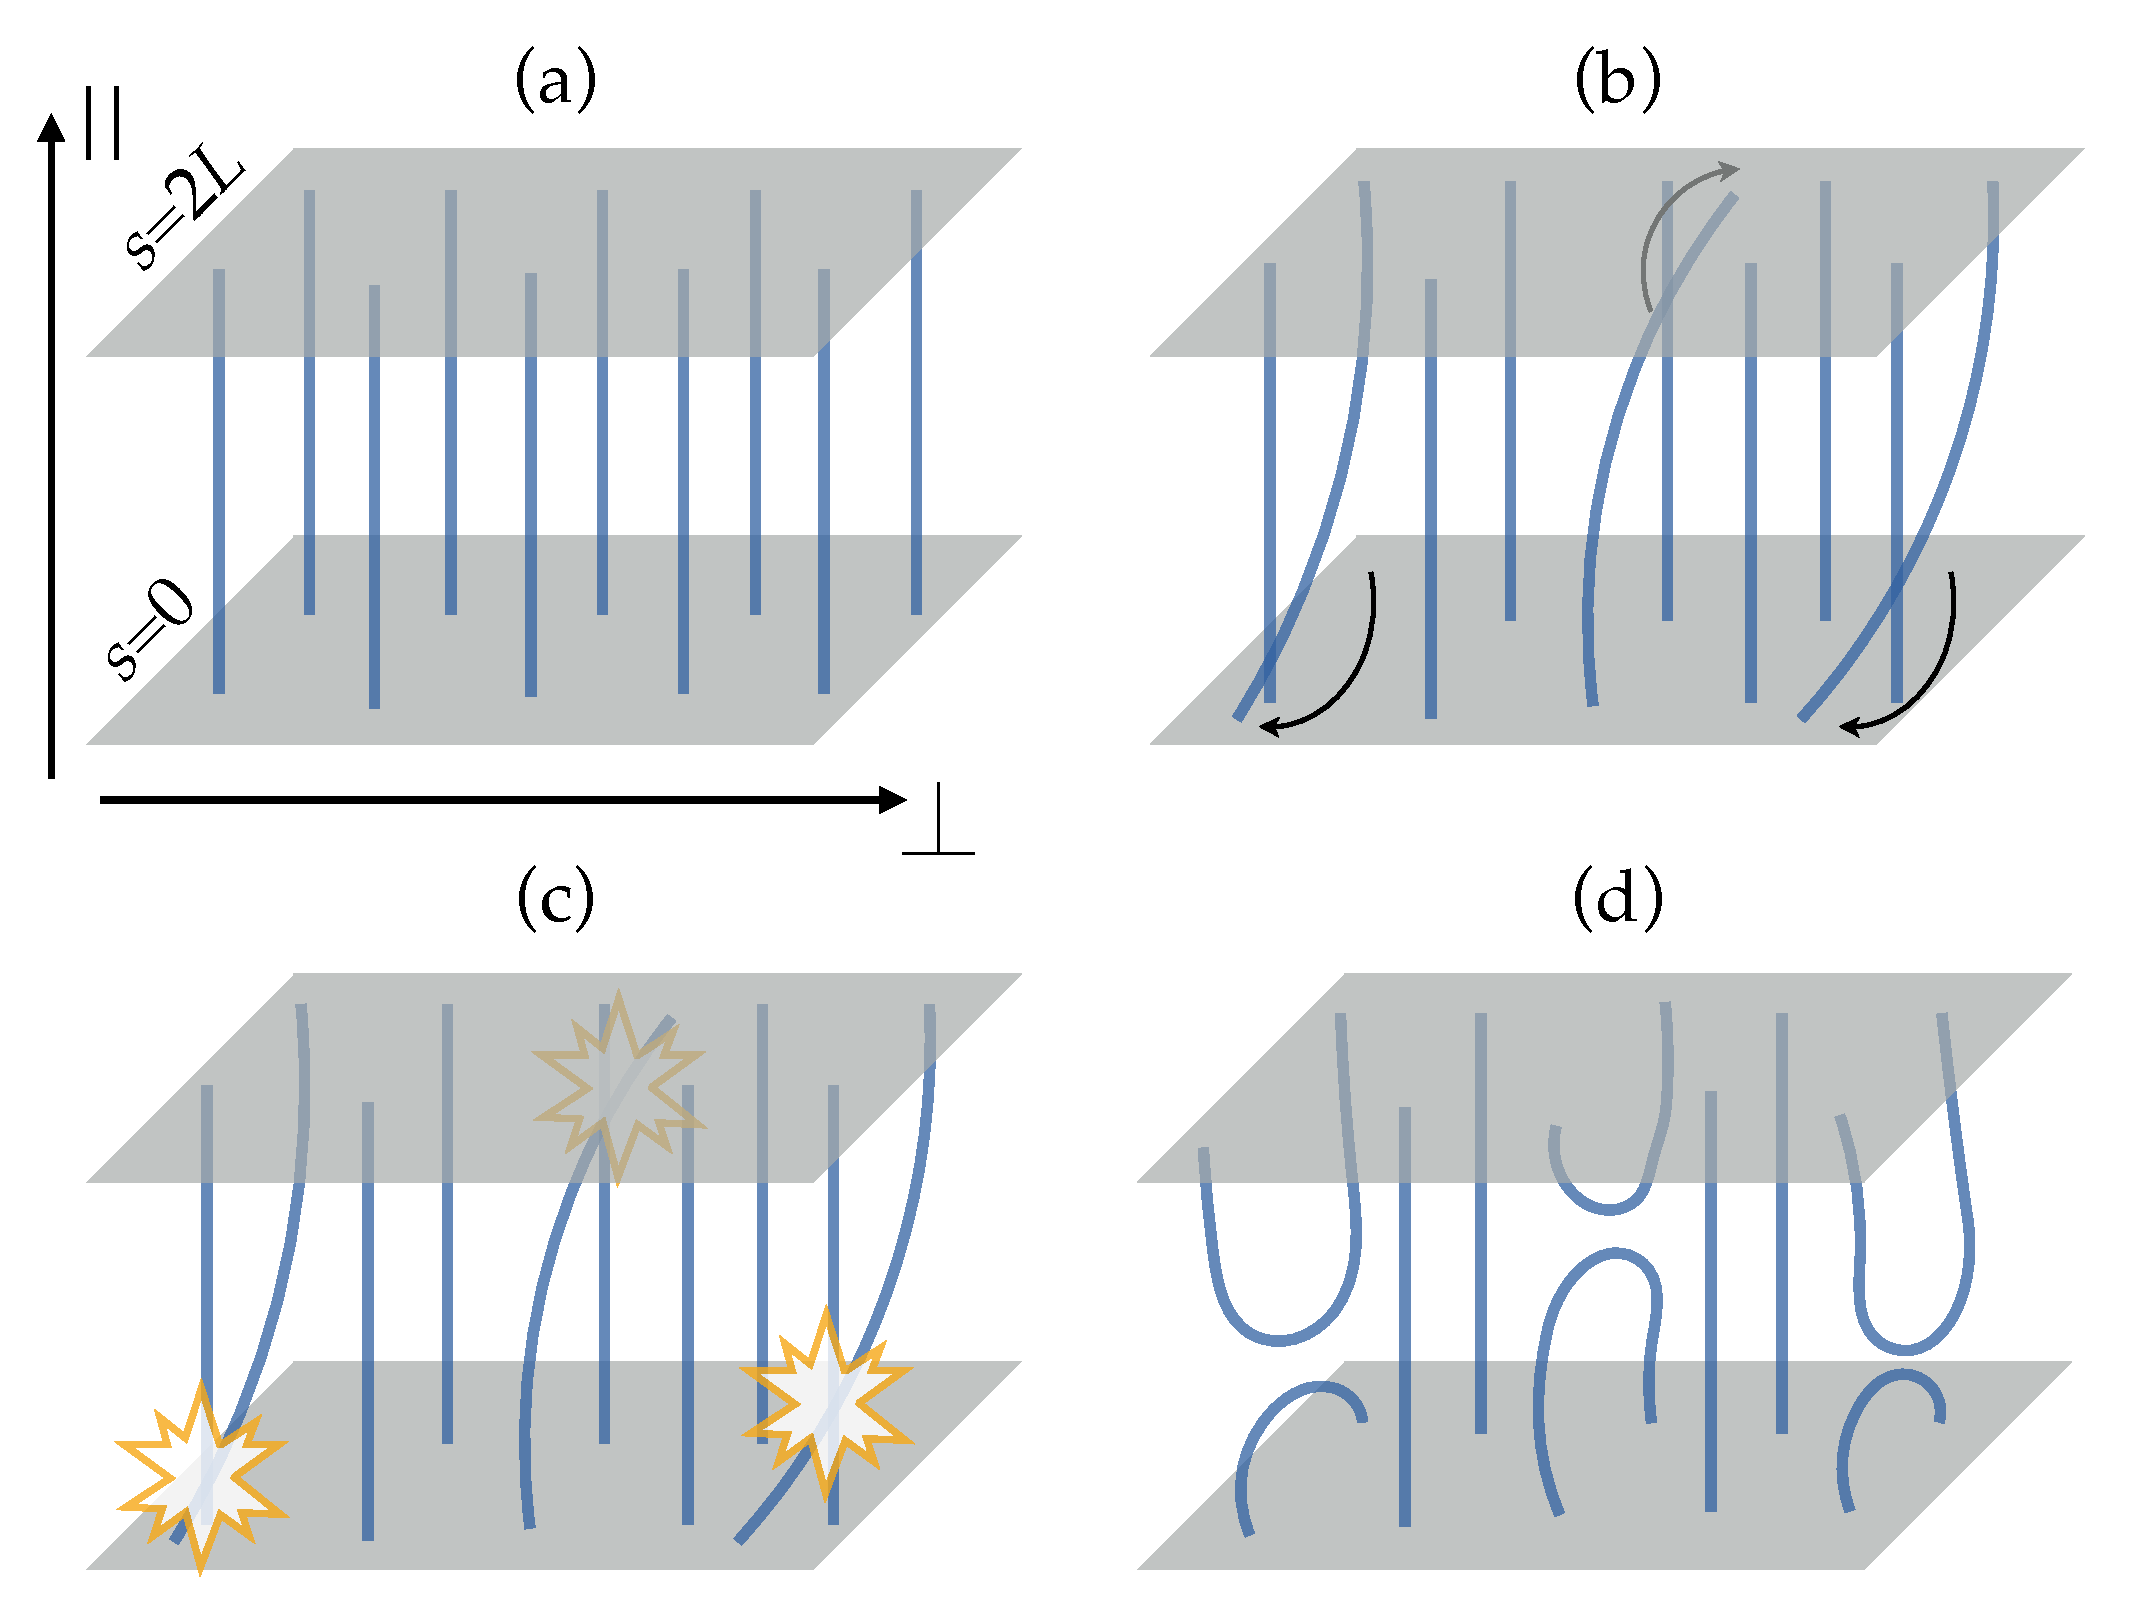
\includegraphics[width=0.75\textwidth]{chapter1/figures/nanoflare-cartoon.pdf}
    \caption{Illustration of the nanoflare heating scenario of \citet{parker_nanoflares_1988}. The flux tubes have been straightened out such that both the top and bottom gray surfaces correspond to the photosphere. Flux tubes in an initially uniform field (a) are braided when their footpoints are shuffled by the underlying convective motions of the photosphere (b). At some critical angle between the braided flux tubes, they reconnect (c) and relax back to some lower energy state (d). The axes in panel (a) indicate the directions parallel and perpendicular to the magnetic field. Adapted from Figures 5 and 7 of \citet{klimchuk_key_2015}.}
    \label{fig:nanoflare-cartoon}
\end{figure}

% spell-checker: disable %
\begin{pycode}[chapter2]
# Estimate critical angle
B_parallel = 1e2*u.G
F = 1e7 * u.erg / u.cm / u.cm / u.s
v = 0.5 * u.km / u.s
theta_c = np.arctan(4*np.pi*F.value/B_parallel.value**2/v.to(u.cm/u.s).value)
theta_c = theta_c * u.radian
\end{pycode}
% spell-checker: enable %

Following \citet{parker_nanoflares_1988}, the nanoflare energy can be estimated as follows. Consider the simplified geometry shown in \autoref{fig:nanoflare-cartoon} in which a flux tube extends from $s=0$ to $s=2L$, where both surfaces correspond to the photosphere and the flux tube has been straightened. Let the footpoint at $s=2L$ be fixed and the footpoint at $s=0$ move randomly across the surface with velocity $v$. The angle $\theta$ between the vertical and the displaced flux tube as a function of time $t$ is,
\begin{equation}
    \tan{\theta(t)} \approx \frac{vt}{2L},
\end{equation}
provided the angle is small (i.e. $\theta(t)<1$). If $B_\parallel$ is the vertical component of the field, the resulting perpendicular component can be expressed as,
\begin{equation}
    B_\perp = B_\parallel\tan{\theta(t)} \approx \frac{B_\parallel vt}{2L}.
\end{equation}
The Poynting flux associated with the work done by the footpoint motion on the field is given by,
\begin{equation}
    F = -\frac{1}{4\pi}B_\parallel\mathbf{B}_\perp\cdot\mathbf{v}_\perp = \frac{B_\parallel^2 v}{4\pi}\tan{\theta(t)} \approx \frac{B_\parallel^2 v^2 t}{4\pi(2L)}.
\end{equation}
For typical \AR{} values of $F=\SI{e7}{\erg\per\square\cm\per\second}$ \citep{withbroe_mass_1977}, $B_\parallel=\SI{100}{\gauss}$, and $v=\SI{0.5}{\km\per\second}$, $\theta\approx\py[chapter2]|f'{theta_c.to(u.degree).value:.0f}'|\si{\degree}$. Once $\theta$, the angle between $B_\perp$ and $B_\parallel$, reaches this critical value, the energy is rapidly dissipated by reconnection and the field relaxes back to its equilibrium state, destroying $B_\perp$. Note that the absence of dissipation and reconnection would result in an infinite build-up of stress in the field \citep{klimchuk_key_2015}.

Furthermore, the energy associated with each of these discontinuities in the field can be written as,
\begin{equation}
    \varepsilon = \ell^2\Delta L \frac{B_\perp^2}{8\pi},
\end{equation}
where $\ell$ is the length of each random step and $\Delta L$ is the length of winding along the neighboring flux tube. Assuming the lifetime of each step is $\approx\SI{500}{\second}$, $\ell=\SI{250}{\km}$ and $\Delta L=\ell/\tan{\theta}=\SI{e3}{\km}$. Thus, the free energy associated with the winding of the field is $\varepsilon\approx\SI{6e24}{\erg}$, in approximate agreement with observations. \citet{parker_nanoflares_1988} notes that the energy of the resulting nanoflare will, on average, be less than this value.

Much progress has been made in understanding the role of nanoflares in heating the solar corona though a definitive detection has yet to be made. Early modeling efforts by \citet{cargill_implications_1994} and \citet{cargill_nanoflare_2004} showed that nanoflares lead to a broad distribution of temperatures and can produce ``very hot'' plasma at temperatures in excess of \SI{8e6}{\kelvin}, the so-called ``smoking gun'' of nanoflare heating. While spectroscopic observations of ``warm'' \SIrange{1}{2}{\mega\kelvin} provide compelling, indirect evidence of impulsively heated plasma \citep[e.g.]{warren_constraints_2011,warren_systematic_2012,viall_evidence_2012}, a direct detection of $>\SI{8}{\mega\kelvin}$ with current instruments is not likely \citet{winebarger_defining_2012}. However, recent results from two sounding rockets, the Extreme Ultraviolet Normal Incidence Spectrograph \citep[EUNIS,][]{brosius_pervasive_2014} and the Focusing Optics X-ray Solar Imager \citep[FOXSI,][]{ishikawa_detection_2017}, provide possible detections of this very hot plasma.

Though the original nanoflare concept of \citet{parker_nanoflares_1988} was explicitly tied to reconnection, the modern definition of a nanoflare is far more general. Throughout the remainder of this thesis, I adopt the definition of \citet{klimchuk_key_2015} that a nanoflare is \textit{an impulsive energy release on a small cross-field spatial scale without regard to physical mechanism}. Nanoflares may be caused by waves or by reconnection as both have been shown to be impulsive \citep{klimchuk_solving_2006,klimchuk_key_2015}. Nanoflare events may occur frequently or infrequently on a given flux tube and their energy spectrum may be broad though it is likely to favor lower energy events \citep{hudson_solar_1991}. Rather than probing a specific physical mechanism, the work in this thesis is focused on constraining the properties of the heating, regardless of the underlying driver.

\section{Aims of this Work}\label{sec:aims}

% Nomenclature
\nomenclature[a-rsun]{$R_{\solar}$}{radius of the Sun, $\approx\SI{6.957e10}{\cm}$}
\nomenclature[z-ar]{AR}{active region}
\nomenclature[z-tr]{TR}{transition region}
\nomenclature[z-mhd]{MHD}{magnetohydrodynamics}
\nomenclature[z-noaa]{NOAA}{National Oceanic and Atmospheric Administration}
\nomenclature[z-pfss]{PFSS}{potential field source surface}
\nomenclature[z-aia]{AIA}{Atmospheric Imaging Assembly}
\nomenclature[z-sdo]{SDO}{Solar Dynamics Observatory}
